\documentclass[12pt,glossary]{dalthesis}
\usepackage{amsmath,graphicx,braket}

\newcommand{\ham}{\mathcal{H}}
\newcommand{\machine}{D-Wave Two\ }
\newcommand{\fid}{\mathcal{F}}

\begin{document}

\title{Compiling Programs for an Adiabatic Quantum Computer}
\author{Elliot Snow-Kropla}
%\date{20 July 2012}

\degree{Master of Science}
\degreeinitial{M.Sc.}
\faculty{Faculty of Science}
\dept{Department of Physics and Atmospheric Science}

\defencemonth{August}\defenceyear{2014}

\supervisor{Dr. Kyriakidis}
\reader{Dr. Labrie}
\reader{Dr. Chapman}

%\nolistoftables

\frontmatter

\begin{abstract}
	A method for compiling programs for adiabatic quantum computers is described, and the resulting programs evaluated on a physically implemented adiabatic quantum machine.  These results are used to characterize the performance of the machine.  The AQC machine is found to perform well on some problems with linear scaling with problem size for some instances, but it performs poorly on others and is unable to solve a 6-variable satisfiability problem at all.
\glossary{name={AQC},description={Adiabatic Quantum Computing}}
\glossary{name={$\fid$},description={The overlap between the target state and measured state at the end of the adiabatic evolution; $|\braket{\psi_{gs} | \psi(T)}|^2$}}
\glossary{name={$\sigma_i^z$},description={The operator for spin along the $z$ axis of the ith particle.}}
\glossary{name={SAT},description={Boolean Satisfiability is an NP-Complete problem, the first such discovered.}}
\glossary{name={\machine},description={The \machine is an machine designed to be an adiabatic quantum computer created by D-Wave Systems}}
\glossary{name={$\alpha$},description={The ratio $M/N$ of clauses over variables in a SAT problem.  For a given k-SAT there is a single $\alpha$ which produces the most difficult problem instances.}}
\glossary{name={Clone Coupling},description={The coupling value that the embedding process uses to ensure different qubits share the same logical value.}}
\glossary{name={\texttt{QCC}},description={The program collection which compiles \texttt{QSM} programs into embeddable Hamiltonians.}}
\glossary{name={\texttt{QSM}},description={A high level language for describing Hamiltonians.}}

\end{abstract}

\printglossary

\begin{acknowledgements}
	I would like to acknowledge the help of my numerous people whose assistance was invaluable in assembling this document, including my supervisor Jordan Kyriakidis, Todd Belote, Aaron Whiteway, Micah McCurdy and Jeff Egger.
\end{acknowledgements}

\mainmatter

\chapter{Introduction}

\section{Classical Computing}

\section{Feynman to Shor}
The initial idea of using quantum mechanics to carry out computation is usually attributed to Feynman \cite{feynman}.

\chapter{Adiabatic Quantum Computing}
\label{chap:aqc}

MAP THE CHAPTER

\section{The Adiabatic Theorem}

The central idea of Adiabatic Quantum Computation is solving problems by finding the ground states of specially constructed Hamiltonians.\cite{farhi}  Ground state relaxation is a form of analog computing where we rely on physics to do the calculating for us: we set up a physical system so that the ground state is the solution to our problem and let the system evolve.  Generally speaking, we expect that classical or quantum systems will still take exponentially long to reach this desired ground state for NP-hard problems.\cite{aaronson}
By starting the system in an easy to prepare state (e.g. ferromagnetically aligned) and then evolving adiabatically into our prepared problem state AQC uses the \emph{adiabatic theorem} to (hopefully) avoid this exponential delay.

The adiabatic theorem states that if a system is initially prepared in the ith energy level $\ket{\psi_i}$, and the Hamiltonian is evolved according to the adiabatic condition, the system will remain in the ith state after the evolution.  The adiabatic condition is:

\begin{equation}
	\left | \frac{1}{\omega_{fi}}\frac{\partial}{\partial t} \braket{\psi_f | \hat{V}(t) | \psi_i} \right | << |E_f - E_i|
\end{equation}

where $E_i$ and $E_f$ are the energies of the initial and final states $\ket{\psi_i}$ and $\ket{\psi_f}$, $\hat{V}(t)$ is the time dependant part of the Hamiltonian and $\omega_{if} = \frac{E_f - E_i}{\hbar}$ is a convenient variable.  For a derivation of the adiabatic theorem see Appendix \ref{apx:aqc}.\cite{zettili}  When the adiabatic condition is satisfied the probability of transition from state $i$ to state $f$ is zero, that is

\begin{equation}
	|\braket{\psi(t\rightarrow\infty)|\psi(t=0)}|^2 \rightarrow 1
\end{equation}

So if the speed at which the Hamiltonian changes (the derivative term) is slow enough, and the gap $\Delta$ between the initial state and the other states ($\Delta = E_f - E_i$) is large enough, then the system won't transition into a new state.  

\section{Finding a Problem Hamiltonian}
\label{sec:prob_ham}
While in principle there are an unlimited number of ways to construct a Hamiltonian whose ground state encodes the solution to a computation, our method is to use an N-particle Hamiltonian of the form
\begin{equation}
	\label{eq:ham}
	\ham_f = \sum_{i} h_i \sigma_i^Z + \sum_{i < j} J_{ij} \sigma_i^Z\sigma_j^Z 
\end{equation}
where $\sigma_i^Z$ is the z-pauli matrix of the ith particle and $h_i$ and $J_{ij}$ are the parameters of the Hamiltonian.  
This 2-local Hamiltonian corresponds to a graph structure, where each particle is a vertex and each non-zero $J_{ij}$ is an edge, while non-zero $h_i$s can be represented as edges to a constant ``field'' spin.

Our problem of finding a suitable Hamiltonian is now reduced to finding a set of $h$'s and $J_{ij}$'s such that our desired solution is encoded in the ground state.  This process is called \emph{embedding} and will be described in more detail in Chapter \ref{chap:embed}.  Something very useful in this process is the \emph{gluing theorem}; this theorem states that if we take two Hamiltonians $G$ and $V$ and combine their fields and couplings, the resulting Hamiltonian's ground states are the combination of the ground states of $G$ and $V$.  This allows us to build up larger Hamiltonians out of smaller sub-pieces, such as building an N-bit adder circuit out of adders and half-adders.

Figure \ref{fig:nand_graph} shows a Hamiltonian graph describing the $h_i$'s and $J_{ij}$'s to encode the logic of a NAND gate.  Because NAND's are universal for classical computation, combining this graph with the gluing theorem allows us to encode the evaluation of any computable function into the ground state of a Hamiltonian of the general form described in Equation \ref{eq:ham}.

\begin{figure}
	\begin{center}
	\scalebox{0.5}{
		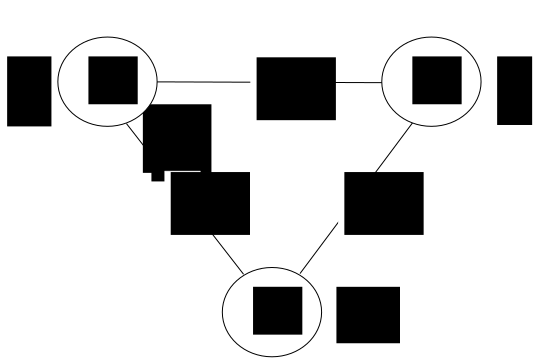
\includegraphics{img/nand.eps}
	}
\end{center}
	\caption[\texttt{NAND} Graph]{Graphical representation of the Hamiltonian implementing the logic of a \texttt{NAND} gate.  Each of the vertices is a spin and the number inside is the field value on that spin; each edge is the coupling value between the respective vertices.  The top two spins are the input spins, while the bottom is the output.  Each ground state of this Hamiltonian enforces the logic $C = \neg(A \wedge B)$.}
	\label{fig:nand_graph}
\end{figure}

Simply evaluating the Hamiltonian depicted in Figure \ref{fig:nand_graph} will reproduce the entire truth table of the \texttt{NAND} gate.  Usually computing the entire truth table of our circuit is not what we want; we want to specify some input and get only the corresponding output.  This is done by a process called \emph{clamping}.  

Clamping manipulates a Hamiltonian to mimic the effect of fixing certain spins to specified values.  This is done in several steps.  First, we select a value $C$ for the spin $s$ to be clamped to.  $s$ is then removed from the Hamiltonian; each coupling between $s$ and a different spin $d$ is removed, and the value $Cs$ is added to the field on spin $d$.  This changes the energy spectrum associated with spin $d$ to match what it would be were $s$ still in the Hamiltonian with the value $C$.

For example, in the \texttt{NAND} Hamiltonian from Figure \ref{fig:nand_graph}, clamping the spin $C$ to $+1$ or $true$  would result in the field terms on $A$ and $B$ becoming $-1 + 1\times2 = 1$.  The final Hamiltonian would then be fields of $+1$ on spins $A$ and $B$ and a coupling between them also with strength $+1$, while $C$ would be gone.  The ground state energy of this Hamiltonian is $-1$, with three ground states corresponding to either spin $A$ or $B$ up with the other down, or both spins down.  The only state of the two spins not in the ground state degeneracy is the state $A = B = \uparrow$; this is the only input to a \texttt{NAND} gate that does not result in a \texttt{true} output, and we restricted this Hamiltonian to values of $A$ and $B$ for which $C$ is \texttt{true}.

The notable feature of this example is that we clamped what is normally an \emph{output} spin.  Because quantum mechanics is reversible, all of our computations must be as well; this means AQC Hamiltonians are symmetric between input and output.  We take advantage of this when designing our circuits: any circuit that computes a function $f$ also computes its inverse $f^{-1}$.  Thus a circuit that computes multiplication is also a circuit that computes integer factorization, depending on whether the spins corresponding to the factors or the multiplicand are clamped.  Since we can construct a classical multiplication circuit out of a polynomial number of \texttt{NAND} gates, we can also construct an AQC integer factorization circuit out of a polynomial number of quantum \texttt{NAND} gates.

\section{Adiabatic Evolution}
Once we have a Hamiltonian whose ground state encodes the problem we would like to solve, we need to set up the evolution.  The Adiabatic Theorem lets us transition from the ground state of one Hamiltonian to another, so we need an initial Hamiltonian.  In general almost any Hamiltonian of which we know the ground state will work.  For simplicity we use the following initial Hamiltonian:
\begin{equation}
	\ham_i = \sum_i^N B \sigma_i^x
\end{equation}
where $B$ is some large constant.  This Hamiltonian has as it's ground state all the spins pointed along the (negative) x-axis (or equivalently, an equal superposition of $\ket{\pm z}$).  This is easy to prepare by applying a large magnetic field along the negative x direction.
Once we've assembled both our initial and final Hamiltonians, we can conduct the evolution.  We call the total Hamiltonian $H_{tot}$, and it is simply the sum of the initial and final Hamiltonian:

\begin{equation}
	\ham_{tot} = A(t)\ham_i + B(t)\ham_f
\end{equation}

where $A(t)$ and $B(t)$ are dimensionless functions of time such that $A(0) = B(T) = 1$ and $A(T) = B(0) = 0$ where $T$ is the final annealing time; this ensures that at $t = 0$ the Hamiltonian is equal to $H_i$ and at $t = T$ the Hamiltonian is equal to $H_f$.  Then the functions $A$ and $B$ describe the \emph{evolution path}.  Combining the evolution path with the speed at which the Hamiltonian is changing (or just the speed), that is $\frac{\partial A}{\partial t}$ and $\frac{\partial B}{\partial t}$, gives us the evolution trajectory.  

Given a ground state of $\ham_{tot}$, $\ket{\psi_{gs}}$, the \emph{fidelity} is the probability of measuring $\psi_{gs}$, or $|\braket{\psi(T)|\psi_{gs}}|^2$.  If there are $N$ correct answer to our computation, and thus $\ket{\psi_N}$ degenerate ground states, the fidelity is defined as

\begin{equation}
	F = \sum_{i=0}^N \braket{\psi(T)|\psi_i}
\end{equation}

For a perfectly annealed system, the fidelity should go to one as the annealing time increases.  Since any real annealing will not be in the infinite anneal time limit, in practice our fidelity values are restricted to be $\leq 1$.  The closer the fidelity is to 1, the more likely our computation is to succeed.  We will use the fidelity later in the experimental results section to evaluate how close we get to ideal AQC.

For a purely quantum mechanical system described by the Hamiltonian $\ham_{tot}$, the evolution trajectory completely determines the fidelity.
The simplest and most obvious trajectory is $A(t) = 1 - t/T$ and $B(t) = t/T$ at a constant speed, or a straight line path through Hamiltonian space.
There is no particular reason that a straight line from $(A=1,B=0)$ to $(A=0,B=1)$ should maximize the fidelity; indeed, because moving away from the origin in Hamiltonian space scales the Hamiltonian and its derived quantities up (including the energy gap), and the adiabatic condition is stated in terms of the energy gap, we expect that some more complicated curve through Hamiltonian space, potentially including changing the evolution speed, will give the best results.

However, in this work we restrict ourselves to evaluating straight line paths through Hamiltonian space due to the adiabatic quantum computer we eventually run jobs on being limited in this manner (see Chapter \ref{chap:machine}).

\section{Simulating AQC}
For small Hamiltonian we can simulate directly the process of quantum annealing by integrating the Schr\"odinger equation. For time dependent Hamiltonians such as ours, the general form of the Schr\"odinger equation is 

\begin{equation}
	i\hbar\frac{\partial}{\partial t} \Psi = \ham\Psi
\end{equation}

this is a linear partial differential equation which can be easily solved by numerical methods.  Using a fourth order Runge-Kutta method\cite{comp_book} we can find the overlap between the ground state $\ket{\psi_f}$ and the current state $\ket{\psi(t)}$ and plot this as a function of the annealing parameter.  Figure \ref{fig:simulate} shows the results of one such simulation.  This shows an eight spin Hamiltonian annealed with linear control parameters $A(t) = 1-t/T$ and $B(t) = t/T$.  The features correspond to what we expect from the adiabatic theorem: the fidelity starts low and climbs as the system evolves.  It does not reach one as we are not in the adiabatic limit because we are annealing for only a finite time.  We expect to see similar results to the one shown here from experimental data; deviations will show us how far our experiments depart from the assumptions of AQC.
\begin{figure}
	\includegraphics{img/simulate.eps}
	\caption[Simulated AQC]{Numerical simulation of adiabatic evolution by integrating the Schr\"odinger equation.}
	\label{fig:simulate}
\end{figure}

%\chapter{Development of Adiabatic Quantum Computing}
\section{Feynman to Shor}
The initial idea of using quantum mechanics to carry out computation is usually attributed to Feynman \cite{feynman}.
\section{Development of AQC}
Adiabatic Quantum Computing was developed initially by E. Farhi and others\cite{farhi}

\chapter{The \texttt{VESUVIUS} Machine}

\chapter{Embedding}
Because in general programs compiled to Ising graphs can be of any shape, we need a way to convert arbitrary graphs into Chimera graphs that can be executed on a machine.  This is done by adding \emph{clone spins} into the graph: each clone spin has the same value in the ground state as one of the logical spins in the input graph.  Thus we can decrease the connectivity of the input graph until it is sparse enough to be isomorphic to a physical machine.  We expect that translating complete graphs onto graphs with constant neighbour counts to require roughly a quadratic size penalty in the number of clone spins (as the number of connection in a complete graph $~ n^2$).
Ideally, to ensure that each clone spin's ground state is the same as it's parent we would have $J_{ij} << J_{clone} \forall i,j$.  Because of physical limits of the machine (especially the resolution mentioned above) large values of $J_{clone}$ may not maximize fidelity: for a machine with finite resolution, having a large $J_{clone}$ may compress other coupling values together such that the ground state starts to overlap with higher energy state.  On the other hand a too small value of $J_{clone}$ may result in ground states in which the clones are not aligned, which will almost certainly also produce incorrect ground states. Thus we have to find an empirical value of $J_{clone}$ that maximizes the fidelity while preserving the ground states.

\section{Embedding algorithm}

The embedding algorithm is as follows:

\emph{\textbf{Definitions:}}

Designate the input Hamiltonian graph $V$ and the output Chimera graph $G$.  Label the spins in $V$ and $G$ as $V_i$ and $G_i$ respectively.
We define the \emph{clone map} $C_i$ as the set of spins $[i,j \ldots]$ which have the same logical value as their parent spin: so for example the clone map of spin 5, $C_5$, might be $[2,3,13]$ which would mean that spins 2, 3, 5 and 13 all share the same logical value.  We define a mapping $M$ between logical spins in graph $V$ and computation spins in graph $G$.  

We also define a \emph{clone coupling} value which is as large as possible and ferromagnetic; this attempts to ensure that all the members of a clone map are aligned in the ground state.  In the final $G$, each member of a clone map should have a clone coupling connecting it to at least one other member of the clone map.

\emph{\textbf{Procedure:}}
\begin{enumerate}
	\item Populate $M$ by mapping each $V_i$ to one of the spins $G_j$ on the left side of a qubyte that lies along the diagonal of $G$
	\item For each field term in $V$, add a field to $G$ on the corresponding spin
	\item For each $J_{ij}$ in $V$, conduct the following operation:
		\begin{itemize}
			\item Scan through both of $C_i$ and $C_j$ to find the pair which are nearest to each other in $G$; call these $x$ and $y$
			\item Get a list of each spin that lies along the path between $x$ and $y$
			\item Assign half of these spins to $C_i$ and half to $C_j$; add the appropriate clone coupling into $G$ for each spin in the path to ensure that the clone map is properly connected
			\item Finally, at the interface between the two new clone map members, add a coupling into $G$ with the same value as $J_{ij}$
		\end{itemize}
\end{enumerate}

Each term in $V$, both fields and couplings, should now have a corresponding term in $G$.  $G$ should also contain many coupling terms that group the necessary clone maps.

This algorithm is tailored AQC machines whose qubits are arranged in a square shape, however, the principle should be easily generalizable: 

\chapter{Boolean Satisfiability}
\section{Satisfiability Problems}
Boolean satisfiability is the problem of determining if there exists an assignment of boolean variables to satisfy a given boolean formula.  A boolean formula is \emph{satisfiable} if there is some assignment of the variables within it that causes the whole expression to evaluate to \texttt{true}, and is \emph{unsatisfiable} if there is no such assignment.  
A boolean expression in conjunctive normal form consists of the conjunction of a set of clauses, each clause consisting of the disjunction of some number of variables (or their negations).  When each clause has $k$ variables, then the problem of finding a satisfying assignment is called $k$-SAT.  An example 3-SAT expression might look like the following

\begin{equation}
	(x_1 \vee x_2 \vee \neg x_3) \wedge (\neg x_1 \vee \neg x_2 \vee \neg x_3) \wedge (x_1 \vee \neg x_2 \vee x_3)
\end{equation}

which has five satisfying assignments:

\begin{center}
\begin{tabular}{l || l | l | l | l | l}
	\multicolumn{1}{l}{} & \multicolumn{5}{c}{Assignments} \\
	$x_1$ & \texttt{T} & \texttt{T} & \texttt{T} & \texttt{F} & \texttt{F} \\
	$x_2$ & \texttt{F} & \texttt{F} & \texttt{T} & \texttt{T} & \texttt{F} \\
	$x_3$ & \texttt{F} & \texttt{T} & \texttt{F} & \texttt{T} & \texttt{F} \\
\end{tabular}
\end{center}

$k$-SAT is NP-Complete\cite{sat} for $k > 2$, and is interesting because it was the first and is one of the most general NP-Complete problems; it is generally very easy to find reductions from other problems into boolean satisfiability.  For this reason we use boolean satisfiability (specifically 3-SAT) for the testing of the \texttt{VESUVIUS} machine.

\section{Randomly Generating 3-SAT Problems}
We can build 3-SAT instances with $N$ variables and $M$ clauses by randomly selecting three elements from the set of $N$ variables and their negations $M$ times.  Care must be taken when choosing $N$ and $M$ however; while 3-SAT is NP-Complete in general, the difficulty of any particular instance depends strongly on the ratio $\alpha = M/N$\cite{Kirkpatrick}.  In the small $\alpha$ regime there are many satisfying assignments, and any algorithm to find a solution will likely stumble on one by chance.  Contrariwise, in the large $\alpha$ regime, there are likely to be \emph{no} satisfying assignments.

As discussed in Kirkpatrick and Selman\cite{Kirkpatrick}, there is a phase transition between the many solution and zero solution regimes, which occurs around the value of $\alpha$ for which there is likely to be one solution.  This is the region where finding a satisfying assignment (or proving there is none) is the hardest, and helps to keep us from falsely believing our algorithm is better than it is due to too easy SATs.  This transition is sharper for larger values of $N$ or $M$, and broader for smaller values.  As the value of $N$ and $M$ that will fit onto the \texttt{VESUVIUS} machine are very small, we don't expect to see a very sharp difference for different values of $\alpha$.  Kirkpatrick and Selman report that for 3-SAT, the transition occurs at $\alpha \sim 4.17$.  Therefore we shall attempt to generate SATS which lie as close to this transition as possible; in practice this usually means around $4.25 \pm 0.25$ due to the fact that $N$ and $M$ must be integers and the size of our hardware graph restricts us to small values of $N$ and $M$.

\section{Embedding 3-SAT}
Embedding 3-SAT problems requires two different uses for the computational spins: each logical variable requires a computational spin, and each clause also requires a computational spin.  This is because we embed each clause as a \texttt{3OR} gate, a 4 computational spin gate where the fourth spin's logical value is the disjunction of the three input spins.  This gate requires an auxiliary spin beyond the computational spins to encode its logic.  Because we know that for a satisfying statement each clause must be satisfied, clamping each clause's output variable completes the 3-SAT \texttt{QSM} construction.  As we have roughly four times as many clauses as variables, each clause shares its variables with many other clauses.  This means that the resulting graph is reasonably close to being a complete graph, so we embed them as if they were and tolerate some inefficiency. 

Since the largest complete graph the hardware graph can embed is 32 spins, the largest SAT problem we could embed at an $\alpha$ close to the phase transition is 6 variables and 25 clauses for an alpha of 4.17; however, as discussed in Section \ref{sec:inop_qubits}, the capability of the \texttt{VESUVIUS} machine during our experiments was actually 29 spins, which is too small for 6 SAT variables plus 25 clauses.  The actual largest SAT embedded was thus 6 SAT variables and 21 clauses.

\chapter{Large Instances}
\label{chap:prelim}

\section{SAT-like Hamiltonian}
\begin{figure}[h]
	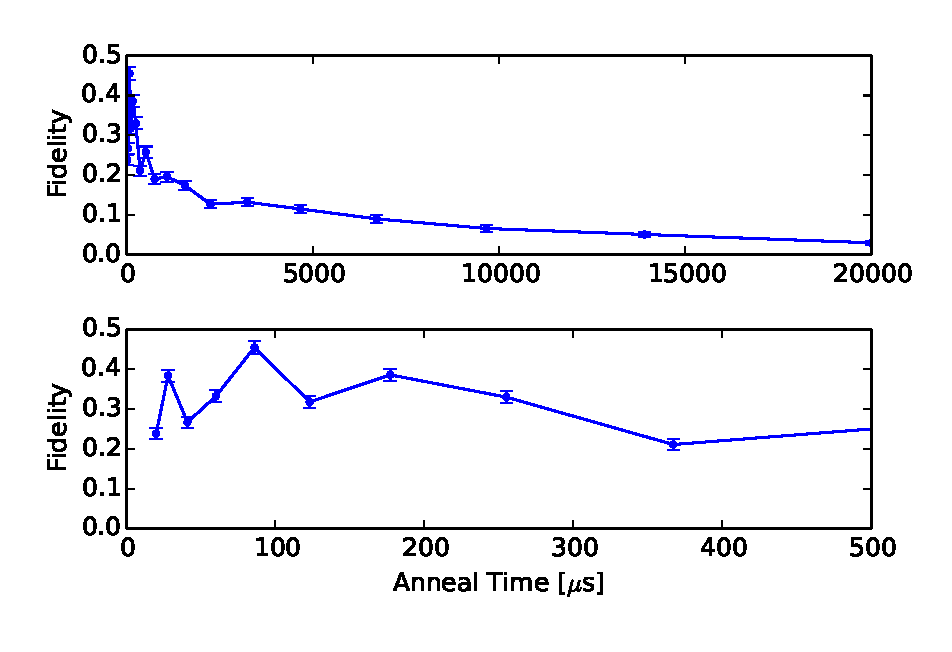
\includegraphics{img/6_018_2_fidelity.eps}
	\caption[Fidelity vs Time]{Plot of the fidelity as a function of annealing time for the Hamiltonian ``6\_018'' for both the full time range and the first 10 time points.  Both windows show the same data set.  Errors are estimated from $\sigma = \sqrt{np(1-p)}$.  Interesting features include the decrease in fidelity with longer anneal time and that the fidelity is very volatile over the short anneal time periods.}
	\label{fig:fidelity}
\end{figure}

Preliminary results were gathered on a sample quasi-random Hamiltonian called ``6\_018''.  This problem Hamiltonian was built up of clusters of clause sub-Hamiltonians in the same way as a SAT solver Hamiltonian would be, although ``6\_018'' does not encode a actual SAT problem.  This Hamiltonian was simple to generate and allowed us to verify our procedure for analyzing AQC results.
Data was collected in a series of evolutions at annealing times ranging from 20 $\mu$s to 20 ms.  Each evolution consists of choosing an anneal time and programming the problem Hamiltonian onto the hardware, then annealing 1000 times successively and reading out the final states.  We call each of these individual evaluations a \emph{read}, and a whole sequence of reads with the same programmed Hamiltonian a \emph{run}.  Any programming error (see \ref{sec:noise}) in the Hamiltonian should be the same between reads and differ between runs.

The state read out after each read is either the ground state, or some other higher energy (and incorrect) state.  The successes and failures thus follow a binomial distribution; there is some probability $p$ of getting the ground state, and probability $1-p$ of getting a different state.
Our best estimate of the fidelity from a single run is thus the fraction of successes, or $p = \frac{gs}{n}$ for $gs$ reads of the ground state and $n$ total reads.  We can also estimate the error in our estimate of the fidelity, because the variance of a binomial distribution is $\sigma^2 = np(1-p)$.

Figure \ref{fig:fidelity} shows the results of an initial set of runs spanning annealing times from 20 $\mu$s to 20 ms.  
There are several features of this data that stand out.  

Figure \ref{fig:short_fidelity} shows the same data as in Figure \ref{fig:fidelity} as well as three more sweeps conducted in the same fashion, annealing out to 500 $\mu$s.  The large-short time oscillations are still seen, and of note is the fact that different runs of the same anneal time lie far outside their respective error margins.  This confirms our earlier suspicion that rather than the quantum annealing fidelity actually changing so rapidly with small changes in anneal time, there is some other uncontrolled factor which is changing from run to run.

\begin{figure}
	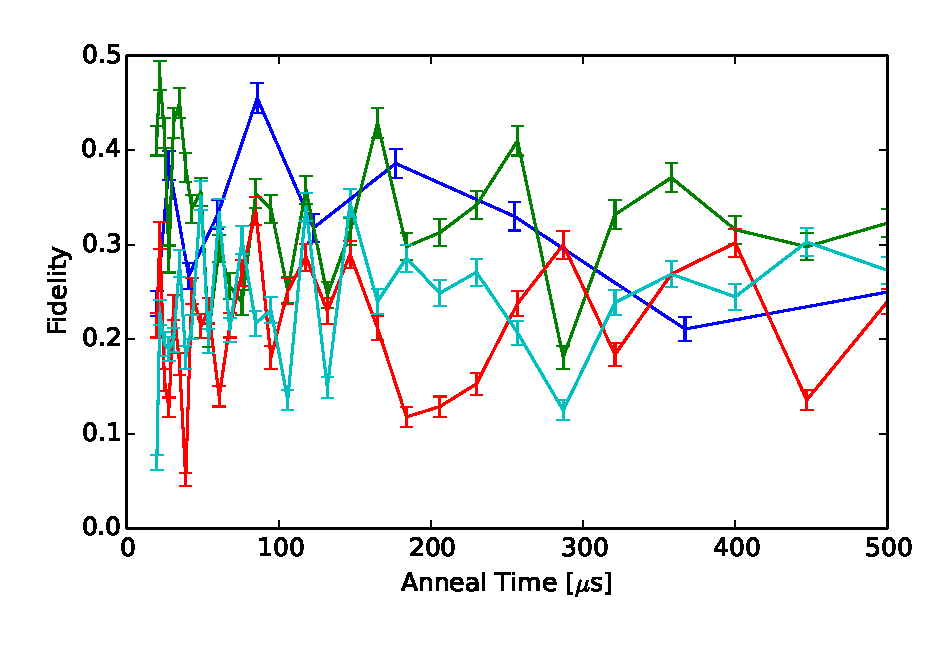
\includegraphics{img/6_018_comparison.eps}
	\caption[Short Time Fidelities]{The fidelity as a function of time for the Hamiltonian ``6\_018'' for several different machine runs.  Each data point consist of 1000 machine reads.  Notice the spread between machine runs is outside of the error bars.}
	\label{fig:short_fidelity}
\end{figure}





Unfortunately there is not much we can do with such low fidelities, so the rest of the results will focus on simpler Hamiltonians such as ones which occupy single K44s.  This means we cannot benchmark the \machine machine to any degree as was the initial plan since actual 3-SAT problems, even those as small as 6 problem variables, are too difficult for the machine to solve reliably.

Having carried out these preliminary results, we have established a framework for evaluating the \machine machine: ascertain the cause of the large uncertainty in the short-time evolution results, using simpler Hamiltonians; measure the effect that number of spins has in a more fine grained manner; and check the intra-run results to see how much of an effect read noise has.


The main Hamiltonian for the rest of the results will be ``k44\_and'', a single qubyte Hamiltonian similar to ``k44'' but featuring only a single non-degenerate ground state.


\begin{figure}
	\scalebox{0.4}{
		\includegraphics[bb= 0 0 1341 868]{img/4th_run_avg_low.png}
	}
	\caption[Running Fidelity Average]{Running average of the fidelity of the Hamiltonian ``6\_018'' for several short-time anneals, showing the change in fidelity with increasing read number.  The number of reads averaged over increases from zero to one thousand.  The rightmost edge of each data set shows the final fidelity estimate for that anneal time.  }
	\label{fig:running_avg}

\end{figure}
\section{Read noise}
First we examine the question of whether there is significant drift in the fidelity within a single run.  That is, does the probability of getting the ground state on any given read depend on the read number (the first read, second read etc.).  This question was examined on the Hamiltonian ``6\_018'' because the data collected on that particular Hamiltonian always consisted of at least 1000 reads per run.
Figure \ref{fig:running_avg} shows the running average of some short-time anneals from a single sweep of ``6\_018''.  If there is not significant read noise, we expect that the running average should flatten out and converge on the ``true'' fidelity after the appropriate number of reads.  For example, for a standard deviation $\sigma = \sqrt{np(1-p)}$ we expect that the running average should be within 5\% of the true fidelity after $\sim$ 200 reads.  Most of the anneal times appear to be reasonably flat past $\sim$ 500 reads, so the running averages appear to indicate to us that there isn't significant read noise (or at least, not nearly enough to be responsible for the short-time oscillations we saw in Chapter \ref{chap:prelim}).

The running average is a somewhat flawed quantity however, since it privileges earlier reads over later ones (since each read contributes like $1/N$ for $N$ reads already counted).  To remedy this we can also look at a rolling average of the fidelity as the reads come in.  Figure \ref{fig:rolling_avg} shows a rolling average of the fidelity for the same data as Figure \ref{fig:running_avg}.  Each point is the ground state fraction of the 100 reads around the labelled point; e.g. the value at point 500 is the number of ground states found from reads 450 to 550 over 100.  The rolling average has an advantage over the running average in that it does not prefer any part of the data set, but it can be harder to make out trends than in the running average.  It can be seen in the rolling average data that there does not appear to be a trend toward the fidelity being higher or lower in different segments of the run; e.g. the 22 $\mu$s run has highest fidelity in the nieghbourhood of read 600, while the 25 $\mu$s run has a minimum in the same location.

The combined results of the running and rolling averages would seem to indicate that intra-run errors, or errors occurring in the process of administering different reads, are not a significant contributor to the final observed fidelity for any given problem.

\begin{figure}
	\scalebox{0.35}{
		\includegraphics[bb=0 0 1582 917]{img/4th_run_roll_avg_low_100.png}
	}
	\caption[Rolling Fidelity Average]{Rolling average of the estimated fidelity for data collected from Hamiltonian ``6\_018'' at the seven shortest anneal times.  Each point is the average fidelity over a one hundred point window, e.g. the value at point 500 is the total number of times the ground state was measured between reads 450 and 550 divided by one hundred.}
	\label{fig:rolling_avg}
\end{figure}

\chapter{Results and Discussion}
\begin{figure}
	\scalebox{0.4}{
		\includegraphics[bb= 0 0 1341 868]{img/4th_run_avg_low.png}
	}
	\caption[Running Fidelity Average]{Running average of the fidelity of the Hamiltonian ``6\_018'' for several short-time anneals, showing the change in fidelity with increasing read number.  The number of reads averaged over increases from zero to one thousand.  The rightmost edge of each data set shows the final fidelity estimate for that anneal time.  }
	\label{fig:running_avg}
\end{figure}
\section{Read noise}
First we examine the question of whether there is significant drift in the fidelity within a single run.  That is, does the probability of getting the ground state on any given read depend on the read number (the first read, second read etc.).  This question was examined on the Hamiltonian ``6\_018'' because the data collected on that particular Hamiltonian always consisted of at least 1000 reads per run.
Figure \ref{fig:running_avg} shows the running average of some short-time anneals from a single sweep of ``6\_018''.  If there is not significant read noise, we expect that the running average should flatten out and converge on the ``true'' fidelity after the appropriate number of reads.  For example, for a standard deviation $\sigma = \sqrt{np(1-p)}$ we expect that the running average should be within 5\% of the true fidelity after $\sim$ 200 reads.  Most of the anneal times appear to be reasonably flat past $\sim$ 500 reads, so the running averages appear to indicate to us that there isn't significant read noise (or at least, not nearly enough to be responsible for the short-time oscillations we saw in Chapter \ref{chap:prelim}).

The running average is a somewhat flawed quantity however, since it privileges earlier reads over later ones (since each read contributes like $1/N$ for $N$ reads already counted).  To remedy this we can also look at a rolling average of the fidelity as the reads come in.  Figure \ref{fig:rolling_avg} shows a rolling average of the fidelity for the same data as Figure \ref{fig:running_avg}.  Each point is the ground state fraction of the 100 reads around the labelled point; e.g. the value at point 500 is the number of ground states found from reads 450 to 550 over 100.  The rolling average has an advantage over the running average in that it does not prefer any part of the data set, but it can be harder to make out trends than in the running average.  It can be seen in the rolling average data that there does not appear to be a trend toward the fidelity being higher or lower in different segments of the run; e.g. the 22 $\mu$s run has highest fidelity in the nieghbourhood of read 600, while the 25 $\mu$s run has a minimum in the same location.

The combined results of the running and rolling averages would seem to indicate that intra-run errors, or errors occurring in the process of administering different reads, are not a significant contributor to the final observed fidelity for any given problem.

\begin{figure}
	\scalebox{0.35}{
		\includegraphics[bb=0 0 1582 917]{img/4th_run_roll_avg_low_100.png}
	}
	\caption[Rolling Fidelity Average]{Rolling average of the estimated fidelity for data collected from Hamiltonian ``6\_018'' at the seven shortest anneal times.  Each point is the average fidelity over a one hundred point window, e.g. the value at point 500 is the total number of times the ground state was measured between reads 450 and 550 divided by one hundred.}
	\label{fig:rolling_avg}
\end{figure}

\section{Short-time oscillations}
Looking to expand on the results of Chapter \ref{chap:prelim}, multiple sweeps of data were collected from a Hamiltonian labelled ``k44\_and''.  Figure \ref{fig:results_avg} shows the resulting fidelity estimates as a function of time.  This Hamiltonian not only occupies a single qubyte like ``k44'', but there is only one unique ground state.  These properties were chosen to attempt to minimize complicating factors.  Runs were carried out at annealing times from 20 $\mu$s to 20 ms as before.  Each run consisted of 100 reads, and 35 different runs were conducted at each anneal time.  Each fidelity estimate consists of a weighted average of each of the individual run estimates, weighted by the binomial error $\sigma$ for that run.
The error estimate at each anneal time is the standard deviation of the distribution of the individual run estimates.

Unlike in Chapter \ref{chap:prelim}, averaging over many runs at the same anneal time has managed to remove the short-time oscillations.  Figure \ref{fig:hist} shows a histogram of fidelities measured for ``k44\_and'' at an anneal time of 20 $\mu$s.  The Gaussian shape suggests that there are two effects going on: first, there is a value of the fidelity determined mainly by the quantum annealing (at the centre of the distribution) and second, that there is some noise applied over the fidelity from run to run.  The most likely source of this seems to be the programming error from imprecision of the physical couplings (see Sections \ref{sec:noise} and \ref{sec:coupling}).  If the noise in programming the couplings is high enough that if two adjacent couplings end up close enough together then the fidelity will drop because instead of the state we expect being the ground state and thus the most common, it will actually be some higher energy excited state and thus if the annealing is carried out successfully will have low probability of being found.  In the other scenario where two adjacent couplings are randomly bounced away from each other, it is entirely possible that in addition to the ground state being correctly encoded the gap is larger, thus increasing the fidelity.

\begin{figure}
	%includegraphics
	\caption[Averaged Anneal Results]{Fidelity vs anneal time with each data point averaged over multiple different runs.  Each run was used to estimate the fidelity independently as in Chapter \ref{chap:prelim}, with the final estimate the weighted average of each run.  The errorbars reflect the standard deviation of the distribution of estimates from each run.}
	\label{fig:results_avg}
\end{figure}

\begin{figure}
	%includegraphics
	\caption[Estimated Fidelity Histogram]{Histogram of the estimated fidelities for each run of the Hamiltonian ``k44\_and'' with an anneal time of 20 $\mu$s.  The shape appears roughly Gaussian, indicating that while there is a random factor in the fidelity that varies from run to run, there is still a central value that we take in this case to be roughly FIXME.}
	\label{fig:hist}
\end{figure}

\begin{figure}
	%includegraphics
	\caption[Fidelity Distribution vs. Time]{This figure shows the breadth of the distribution of estimated fidelities, i.e. the standard deviation $\sigma$ as a function of the annealing time for the Hamiltonian ``k44\_and''.  As the annealing time increases, the short-time oscillation effect observed in the preliminary results dies off and the distribution narrows.}
	\label{fig:std_time}
\end{figure}

Figure \ref{fig:std_time} shows the standard deviation of the fidelity estimates from evaluation of ``k44\_and'' as a function of the annealing time.  As we saw in the previous results, the large oscillations observed in the short-time fidelity die away as the annealing time increases.  This quantifies our earlier observation of the short-time oscillations: there are two regimes of the annealing, one below $\sim 500$ $\mu$s where the standard deviation is $\sim$ FIXME and one above $\sim 500$ $\mu$s where the standard deviation quickly drops down to FIXME.

This still does not explain \emph{why} the short-time oscillations do not persist into longer annealing times.  The above argument regarding overlap of the physical couplings applies just as well to annealing at longer times.

\section{Clone coupling value}
\label{sec:coupling}
As discussed in Sections \ref{sec:embed_algo} and \ref{sec:resolution}, while for an ideal machine maximizing the clone coupling value would ensure that adding clones did not alter the ground states of our problem Hamiltonians, the \texttt{VESUVIUS} machine can only implement 15 different clone coupling values.  In addition, these values must be evenly spaced.  If we were to use a clone coupling value of $-14$ in a problem Hamiltonian which natively had coupling values of $-2,-1,1,2$, this would result in compressing each of the positive and negative couplings into one machine value.  The machine only implements couplings of the form 
\begin{equation}
	\pm\frac{x}{7}, 1 \le x \le 7
\end{equation}
so the above example would result in a physically implemented Hamiltonian of $-1/7, -1/7, 1/7, 1/7$ in addition to the clone coupling of $-1$.  Most of the time this will result in a malformed Hamiltonian with incorrect ground states.

In addition to incorrect ground states, it is possible that the programming error in the machine is large enough to make the couplings $1/7$ and $2/7$ close enough to be likely to collide, whereas $1/7$ and $3/7$ could be far enough apart to be programmed correctly every time.  This could mean that even in scenarios where \texttt{VESUVIUS} has enough range to encode the problem Hamiltonian couplings correctly with a large clone coupling value we still don't want to do so.

This means that when selecting a clone coupling value we must balance these two competing factors, the desire to make the clone coupling as large as possible from a Hamiltonian correctness standpoint, and the desire to make it as small as possible from a machine resolution viewpoint.  The Hamiltonian correctness issue is correctness and knowable at the time the Hamiltonian is constructed; however in general to know whether a given clone coupling is large enough or not requires diagonalizing the Hamiltonian, and if this were possible then that would enable us to solve the initial computational problem directly.
The machine resolution problem is not necessarily the same from run to run; it could be that the compression of the problem Hamiltonian caused by the clone coupling value only makes it more likely for the machine to end up in an excited state.

To empirically examine the impact of the value of the clone coupling, the ``k44\_and'' Hamiltonian was embedded multiple different times with a clone coupling value ranging from -1 to -14 (from the smallest coupling in the problem Hamiltonian to twice the native resolution of the machine).  Figure \ref{fig:clone_coupling} shows the results of annealing these Hamiltonians from 20 $\mu$s to 20 ms.  Not only does fidelity increase as the clone coupling value is decreased, the short-time oscillations that we saw in Chapter \ref{chap:prelim} are removed.  At longer anneal times the difference in fidelity is reduced, and the same long-time drop in fidelities that was observed in other Hamiltonians continues.  This means that the mechanism for the long-time fidelity drop is not strongly impacted by the clone coupling value, which is what we would expect.

This provides more evidence that the short-time oscillations are caused by programming error in the \texttt{VESUVIUS} machine; if two couplings in the problem Hamiltonian are compressed together the correct ground states could still be formed in the resulting physical Hamiltonian if the couplings were randomly perturbed in the right directions, but this process would be random and differ greatly from run to run.

\begin{figure}
	%\includegraphics{}
	\caption[Variable Clone Coupling Fidelity]{The change in fidelity as the clone coupling value is scaled from -1 to -14.  The top view shows the scaling over the full time range 20 $\mu$s to 20 ms, while the bottom shows the same data zoomed in on the times 20 $\mu$s to 500 $\mu$s.  The fidelity increases with reducing clone coupling value, but using too small of a clone coupling value can result in incorrect ground states.}
	\label{fig:clone_coupling}
\end{figure}

\section{Size scaling}
The final property studied was the size scaling behaviour of the \texttt{VESUVIUS} machine.  This is 

\chapter{Conclusion}
A variety of Hamiltonians were constructed and evaluated on the \machine hardware.  We have seen several general methods for embedding problems into a form suitable for evaluation on an adiabatic quantum computer at a modest overhead, although even that overhead is a stiff price to pay on the current generation of adiabatic hardware.  While the machine is able to solve single clause SAT problems and other small (8 qubit) problems, a real (still small) problem of 6 SAT variables was too difficult. The machine \emph{was} able to solve a similar number of qubits when the SAT was simple (the ``k44\_and'' case), so the difficulty of the 6 variable SAT must not be purely based on the number of qubits.  

In the process of solving these problems we discovered several factors important for using the D-Wave family of adiabatic machines.  Among them the fact that contrary to expectations shorter anneal times give better results, and that the limited number of built in machine couplings requires careful thought when embedding to ensure that coupling collisions do not occur.


\bibliographystyle{plain}
\bibliography{eskthesis}
\appendix
\chapter{The Adiabatic Theorem}
\label{apx:aqc}

\chapter{Shor's Algorithm}
\label{apx:shor}


\end{document}
